\chapter{State of the art}\label{cha:stateOfTheArt}

The problem statement (\cref{sec:problemStatement}) presents four questions for this project. The \ref{PS:Q:Feasibility} question being the primary question, from which the other three decends. 

To answer the \ref{PS:Q:Feasibility} question we have to identify the key services performed by the Wind Power Supervisor and the Park Pilots. These services must be provided by the new decentralized system such that removing the central control points, the Wind Power Supervisor and the Park Pilots, will not diminish the new decentralized systems function compared to the current system as described by the Siemens Case in \cref{sec:SiemensCase}. The following key services has been identified:

\begin{enumerate}[label=\textbf{\alph*.}, ref=\textit{\alph*}]
\item \label{Analysis:need:a} \textbf{Data aggregation} \\
	It must be possible to aggregate data across the entire wind farm in order to enable calculation of global parameters such as global power production, global max power production etc. 

\item \label{Analysis:need:b} \textbf{Data storage} \\
	The individual turbines must be able to store data about wind speeds, individual power production as well as the state of wear on different parts of the turbine. Several data points are measured every second. As well as individual data, global data must be stored as well. Without a central storage point the global data must be distributed across the entire wind farm such that it is accessible by any turbine handling an external connection which may request such global data.

\item \label{Analysis:need:c} \textbf{External communication} \\
	The wind farm must be able to handle communication with the external world. Currently this is handled by both the Wind Power Supervisor and the Park Pilots depending on which data is relevant to the initiator of the external connection. The external communication must be handled by the turbines of the wind farm such that it is transparent to the initiator which node is actually performing the services requested.

\item \label{Analysis:need:d} \textbf{Park regulation} \\
	The wind farm must regulate the power production towards a global power production setpoint. Without a central controller to calculate the individual setpoints for all turbines these calculations must be done by each individual turbine.
	
\end{enumerate}

For the wind farm to be able to handle the needs above and act as a single unit, we are forced to look at decentralized software components. 

The following chapters describes, analyses and discusses solutions to the needs above. The chapters are divided based on the components we see as solutions to \ref{Analysis:need:a}-\ref{Analysis:need:d}. As such this analysis contains the following chapters:

\begin{enumerate}[label=2.\arabic*]
\item{\textbf{Database storage.}} The obvious solution for need \ref{Analysis:need:a} and \ref{Analysis:need:b}.
\item{\textbf{Load balancing.}} In the decentralized system, the turbines needs to be able to handle need~\ref{Analysis:need:c}. Currently Siemens wind farms can have up to 100 concurrent connections. In order to avoid a single turbine having to handle and process 100 concurrent connections, load balancing has to be introduced to the system.
\item{\textbf{Distributed computing.}} For the turbines to be able to perform park regulations, communication between the turbines is essential, since park regulation demands knowledge about every turbine in the farm. Distributed computing is introduced to the system as a way to keep a global state as a solution to need~\ref{Analysis:need:d}. This chapter also addresses problem~\ref{PS:Q:Scalability} of the problem statement.
\end{enumerate}

Problems \ref{PS:Q:Availability} and \ref{PS:Q:Performance} of the problem statement are addressed by all of the chapters mentioned above.

%Problem -> Alternativer -> Sammenligning -> Endeligt valg
%
%
%Opdeling vs. samme emne
%\begin{itemize}
%\item Vidensudveksling er vigtig
%\item  Opsplitning med undervisning
%\end{itemize}
%
%
%noter:
%pup/sub pattern vs DSM (Distributed shared memory)
%ved multicast operationer fejler mange pup/sub systemer da de bruger almindelige unicast protokoller og derfor sender samme pakke flere gang til forskellige modtagere istedet for at multicast pakken en gang til all. (speciale rapport kilde: Unders\o gelse af Distributed Shared Memory performance og anvendelse ...)
%
%


\section{Database storage}
\label{sec:databaseStorage}
Data storage is vital to a wind farm in order to keep track of the wear of turbine parts, and to persist production and sensor data for later use.
Currently data is aggregated from each turbine and stored on a central node.
This node will over time aggregate hundreds of gigabytes of information.
The data on the node is secured by backup but it is still a single point of failure.
Take out the data storage node or the communication to it and gigabytes of valuable information may be lost.

By distributing the data of the system between all the connected nodes the wind farm will achieve higher availability because the data is present on many different nodes.
Should a node become unavailable another node can communicate the same data.

This chapter contains a description of a number of relevant data storage technologies and a discussion of which technology is the best suited for a system like the Siemens case presented in \cref{sec:SiemensCase}.

Storage technologies will be compared on a set of parameters that are relevant to the case presented in \cref{sec:SiemensCase}. The parameters are presented below in prioritized order:

\begin{enumerate}
\item \textbf{Scalability} \\
The storage technology must be able to scale horizontally in order to allow a varying number of nodes.

\item \textbf{Availability} \\
The data in the system must be available for processing at any time.

\item \textbf{Replication} \\
The data in the system must be replicated between nodes in order to avoid data loss should one node be damaged.
\item \textbf{Failover} \\
The data storage technology must be able to seamlessly switch from a damaged node to a working node if a failure occurs.

\item \textbf{Sharding} \\
The data storage technology must support automatic partitioning of datasets that are larger than the physical storage on one node.

\item \textbf{Aggregation} \\
The data storage technology must support aggregation of data.
\end{enumerate}

\subsection{Relational storage, SQL}
\label{sec:sql}
The traditional way of storing data is in a Relational Database Management System(RDBMS).
These databases rely on a schema to arrange data in tables and their relations.
Using SQL it is easy to query data and to do aggregate operations.
RDBMSs support ACID transactions which ensures operations in the database are processed reliably.

%A shortcoming of the RDBMSs is the problem with object-relational mapping also known as the Impedance Mismatch Problem\cite{Fowler:IntroNoSQL, Neward:TheVietnamOfComputerScience}.
%The relational structure of the RDBMSs does not map well to the object-oriented structure the most popular programming languages encourage.
%Often an object is an aggregate of a number of attributes.
%In the context of the object-oriented program the object is seen as one entity.
%In the context of the RDBMS the attributes of the object-oriented object is often scattered between multiple tables in the database to ensure consistency and avoid duplicate data.
%This mismatch between object representation and relational representation can cause both performance problems, the JOIN operation in SQL is very costly, as well as considerable development time spent mapping one structure to the other.
%The performance problem multiplies in a distributed database if the RDBMS must do JOIN operations across the network in order to aggregate data.

A problem with a traditional RDBMS is that they are designed for vertical scaling~\cite{Atzeni:TheRelationalModelIsDead}. If a traditional RDBMS cannot handle the amount of data it is supposed to the solution is to add a bigger harddrive or invest in a faster CPU. This makes sense in a world were hardware is very expensive like it was when the traditional RDBMSs saw the light of day~\cite{Stonebraker:TheEndOfAnArchitecturalEra}. Today horizontal scaling is preferred. If a system has a problem with the data load, add another machine or add five others if that is what it takes. Since horizontal scalability is a very important feature of the data storage system the traditional RDBMS is not a viable option.

\subsection{Schema-less storage, NoSQL}
\label{sec:nosql}
Since 2009 the schema-less storage methods have become increasingly popular.
Relational databases could no longer keep up with the task of storing and querying big data.
A new breed of schema-less storage systems became popular because they could handle some of the problems big data caused for the relational storage systems.
This new breed of databases are designed for horizontal scalability and without strict schemas allowing a more flexible data model. 
They are capable of handling large scale amounts of data both for data storage but also for analysis or batch operations.
The downside however is the lack of the ACID properties which results in decreased consistency and the lack of transactions. %TODO: Dårligt formuleret omskriv!

The schema-less databases can be divided roughly into four categories~\cite{Fowler:IntroNoSQL, Moniruzzaman:NoSQLDatabaseNewEraOfDatabasesForBigDataAnalysis}:

\begin{itemize}
	\item \textbf{Document databases} \\
	The document databases are primarily used to store semi structured data in the form of documents. The data is stored in attribute name-value pairs, where the attributes may vary between rows.
	
	\item \textbf{Key-value databases} \\
	The key-value databases are primarily used for fast lookup of data based on a key. The data is stored in key-value pairs.
	
	\item \textbf{Column-family databases} \\
	The column-family stores are primarily used for distributed data storage, batch processing of data and analytical processing for statistical use. The data is stored as key-value pairs where the value part contains columns of related data.
	
	\item \textbf{Graph databases} \\
	Graph databases are primarily used to describe relationships between data. Data is stored as nodes and edges. Nodes contain key-value pairs of data and edges describe the relationship between nodes.
\end{itemize}

%\subsubsection{Document databases}
%The document databases are designed to contain documents.
%The documents contains attribute name/value pairs.
%Attributes may vary between rows.
%To retrieve data it is possible to search both on the attribute and the value.
%
%Primary use include storing actual documents like emails and blog posts, or storage of semi-structured and aggregate data.
%
%\begin{figure}
%	\centering
%
%	\begin{tikzpicture}
%		\node[draw, rectangle, minimum height=4.5cm] (a) {
%			\begin{tabular}{c l}
%				\{ & \\
%				& ``ID'': 1, \\
%				& ``Firstname'': ``Thomas'', \\
%				& ``Lastname'': ``Steffensen'', \\
%				& ``Age'': 27, \\
%				& ``Zip'': ``8000'', \\
%				& ``City'': ``Aarhus'' \\
%				\} &
%			\end{tabular}};
%	\end{tikzpicture}
%
%	\captionsetup{format=plain,font=footnotesize,labelfont={bf,defaultCapFont},labelsep=quad,singlelinecheck=no}
%		\caption[Document store]{
%			\label{fig:DocumentStore}
%			\footnotesize{%
%				Document store structure.
%			} 
%	}
%\end{figure}
%
%% \begin{figure}
%% 	\centering
%% 	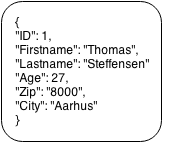
\includegraphics[scale=0.8]{Document.png} 
%% 	\captionsetup{format=plain,font=footnotesize,labelfont={bf,defaultCapFont},labelsep=quad,singlelinecheck=no}
%% 	\caption[Document store]{
%% 		\label{fig:DocumentStore}
%% 		\footnotesize{%
%% 			Document store structure.
%% 		} 
%% 	}
%% \end{figure}
%
%\subsubsection{Key-value stores}
%The key-value stores can be compared to a hashmap since every entry has a key and an associated value. 
%To retrieve data you search for the key. 
%The values can contain any kind of data from simple text to lists or documents.
%
%Primary use includes fast lookup for instance for user sessions or product lists.
%
%\begin{figure}
%	\centering
%
%	\begin{tikzpicture} [
%			diagram item/.style={
%				minimum width=3cm,
%				minimum height=1cm,
%				draw,
%				rectangle
%			}
%		]
%		\node[diagram item] (a) {Key: User1};
%		\node[diagram item, right=.5cm of a] (b) {Value: Stefan};
%
%		\node[diagram item, below=.2cm of a] (c) {Key: User2};
%		\node[diagram item, right=.5cm of c] (d) {Value: Thomas};
%
%	    \draw[arrows=->] (a) to (b);
%	    \draw[arrows=->] (c) to (d);
%	\end{tikzpicture}
%
%	\captionsetup{format=plain,font=footnotesize,labelfont={bf,defaultCapFont},labelsep=quad,singlelinecheck=no}
%		\caption[Key-value store]{
%			\label{fig:KeyValueStore}
%			\footnotesize{%
%				Key-value store structure.
%			} 
%		}
%\end{figure}
%
%% \begin{figure}
%% 	\centering
%% 	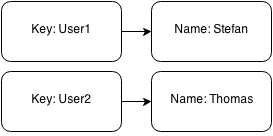
\includegraphics[scale=0.8]{KeyValue.png} 
%% 	\captionsetup{format=plain,font=footnotesize,labelfont={bf,defaultCapFont},labelsep=quad,singlelinecheck=no}
%% 	\caption[Key-value store]{
%% 		\label{fig:KeyValueStore}
%% 		\footnotesize{%
%% 			Key-value store structure.
%% 		} 
%% 	}
%% \end{figure}
%
%\subsubsection{Column-family stores}
%Column-family stores keep related data stored together.
%A column-family object consists of a key-value pair where the value contains columns of related data.
%
%Primary use includes distributed data storage, batch processing of data and analytical processing for statistical use.
%
%\begin{figure}
%	\centering
%
%	\begin{tikzpicture} [
%			diagram item/.style={
%				minimum width=3cm,
%				minimum height=1cm,
%				draw,
%				rectangle
%			},
%			diagram bigitem/.style={
%				minimum width=3cm,
%				minimum height=2cm,
%				draw,
%				rectangle
%			}
%		]
%
%
%		\node (a) {Row key};
%		\node [right=5.7cm of a] (b) {Columns};
%		\node[diagram bigitem, below=0cm of a] (c) {User1};
%		
%		%Attribute names
%		\node[diagram item, right=1.5cm of c, anchor=south] (d) {Firstname};
%		\node[diagram item, right=0cm of d] (e) {Lastname};
%		\node[diagram item, right=0cm of e] (f) {Age};
%		\node[diagram item, right=0cm of f] (g) {Zip};
%
%		%Attribute values
%		\node[diagram item, below=0cm of d] (h) {Thomas};
%		\node[diagram item, below=0cm of e] (i) {Steffensen};
%		\node[diagram item, below=0cm of f] (j) {27};
%		\node[diagram item, below=0cm of g] (k) {8000};
%
%		\node[diagram bigitem, below=.2cm of c] (l) {User2};
%		
%		%Attribute names
%		\node[diagram item, right=1.5cm of l, anchor=south] (m) {Firstname};
%		\node[diagram item, right=0cm of m] (n) {Zip};
%
%		%Attribute values
%		\node[diagram item, below=0cm of m] (o) {Thomas};
%		\node[diagram item, below=0cm of n] (p) {8000};
%	\end{tikzpicture}
%
%	\caption[Column-family store]{
%		\label{fig:ColumnFamilyStore}
%		\footnotesize{%
%			Column-family store structure.
%		} 
%	}
%\end{figure}
%
%% \begin{figure}
%% 	\centering
%% 	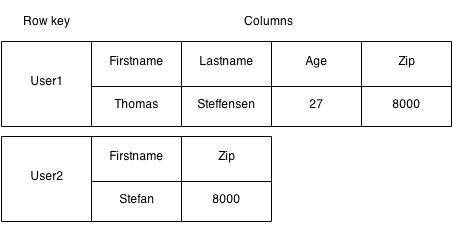
\includegraphics[scale=0.8]{ColumnFamily.png} 
%% 	\captionsetup{format=plain,font=footnotesize,labelfont={bf,defaultCapFont},labelsep=quad,singlelinecheck=no}
%% 	\caption[Column-family store]{
%% 		\label{fig:ColumnFamilyStore}
%% 		\footnotesize{%
%% 			Column-family store structure.
%% 		} 
%% 	}
%% \end{figure}
%
%\subsubsection{Graph databases}
%Graph databases divides data according to nodes and relations between nodes.
%Each node in the graph contains key-value pairs of data, and each edge describes a relationship to another node.
%Graph databases are optimized for traversal of relationships between nodes, not for data aggregation or analysis.
%
%Primary use includes pattern detection and mapping of networks.
%
%\begin{figure}
%	\centering
%	\begin{tikzpicture} [
%			diagram item/.style={
%				minimum width=5.3cm,
%				minimum height=1.5cm,
%				draw,
%				rectangle
%			}
%		]
%
%		\node[diagram item] (a) {
%			\begin{tabular}{rl}
%				Firstname:&Thomas \\
%				Lastname:&Steffensen
%			\end{tabular}};
%
%		\node[diagram item, right=3 of a] (b) {
%			\begin{tabular}{rl}
%				Firstname:&Stefan \\
%				Age:&27
%			\end{tabular}};
%
%		\node[diagram item, below=3 of a] (c) {
%			\begin{tabular}{rl}
%				Firstname:&Mette \\
%				Occupation:&Student
%			\end{tabular}};
%
%		\node[diagram item, right=3 of c] (d) {
%			\begin{tabular}{rl}
%				Name:&Aarhus Universitet
%			\end{tabular}};
%
%		\path (a) -- node[sloped] (knows) {knows} (b);
%		\path (a) -- node[sloped] (married) {married to} (c);
%		\path (a) -- node[sloped] (studies1) {studies at} (d);
%		\path (b) -- node[sloped] (studies2) {studies at} (d);
%
%	    \draw[->] (a)--(knows)--(b);
%	    \draw[->] (a)--(married)--(c);
%	    \draw[->] (a)--(studies1)--(d);
%	    \draw[->] (b)--(studies2)--(d);
%	\end{tikzpicture}
%\end{figure}
%
%% \begin{figure}
%% 	\centering
%% 	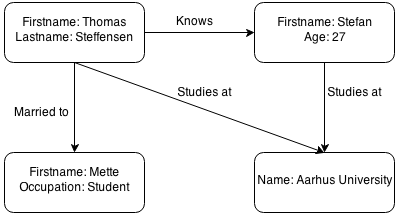
\includegraphics[scale=0.8]{Graph.png} 
%% 	\captionsetup{format=plain,font=footnotesize,labelfont={bf,defaultCapFont},labelsep=quad,singlelinecheck=no}
%% 	\caption[Graph store]{
%% 		\label{fig:GraphStore}
%% 		\footnotesize{%
%% 			Graph store structure.
%% 		} 
%% 	}
%% \end{figure}

\subsection{Relational storage that scale, NewSQL}
\label{sec:newsql}
NewSQL data stores aim to bring the relational data model into the world of horizontal scalability and flexible data models while maintaining the ACID properties and transactions of the traditional RDBMS~\cite{Cattell:ScalableSQLAndNoSQLDataStores}.
This is obtained by implementing a completely new architecture~\cite{CORBETT:SpannerGooglesGloballyDistributedDatabase}.
Starting from nothing with a new architecture allows the NewSQL data stores to be designed to take advantage of the distributed paradigms and to incorporate more flexibility into the schema structure.
The key differences between traditional SQL data stores and the NewSQL data stores are therefore found in the way the NewSQL data stores are built for scalability and throughput.
They try to avoid the major performance barriers which are locking, write-ahead logging, buffer pool overhead and latching~\cite{Stonebraker:NewSQLvsNoSQLForNewOLTP}.

Locking can be avoided by performing transactions in timestamp order or using multi version concurrency control.
Write-ahead logging can be avoided by doing automatic replication and failover.
To avoid buffer pool overhead the NewSQL data stores can run in main memory, either entirely or have a hot store in memory for active data and a cold store on disk for stale data.
To avoid latching transactions can be run single-threaded, meaning transactions must run to completion without descheduling.

Using some or all of these upgrades the NewSQL data stores can achieve higher throughput than the traditional SQL data stores.
Other features like distributed concurrency control and distributed query processing allows the NewSQL data stores to scale horizontally.

NewSQL data stores are divided into three categories~\cite{Prasanns:NewSQLTheNewWayToHandleBigData}:

\begin{itemize}
\item New databases: Completely new systems designed for scalability and throughput.
\item New MySQL storage engine: Keep the existing MySQL interface and redesign the storage engine in order to achieve scalability.
\item Transparent clustering and sharding: Provide extra features for transparent clustering and sharding on top of existing database systems. 
\end{itemize}

\subsection{SQL, NoSQL or NewSQL?}
This thesis aims to create a decentralized system with scalability and redundancy as the most important parameters.
This means that traditional SQL is not an option because of the poor scalability.

NoSQL and NewSQL has clear advantages because they are built as a consequence of the shortcomings of the traditional database systems when it comes to decentralized systems.
NoSQL has the advantage of high scalability and high throughput on data analysis, but the cost is a lack of ACID and transactions.
NewSQL promises to keep the ACID properties and transactions of the traditional database systems while simultaneously allowing horizontal scalability and high throughput.

Since both NoSQL and NewSQL seems like fitting technologies for data management in the Siemens case a further comparison between two state of the art implementations must be done in order to decide which technology will be the best suited.

\subsection{State of the art NoSQL}
To identify state of the NoSQL and NewSQL databases the website \inlineURL{db-engines.com}~\cite{db-engines} is used.
This website maintain a list of more than 200 different databases ranked by popularity. The list is updated monthly based on search engine popularity, discussion threads, job-offers, mentions on LinkedIn and tweets. This does not give the complete and objective ranking but it gives a pointer to the most popular database in their respective category.

Since we expect a stream of measured values from a wide range of parameters on every turbine a key-value store seems to be the obvious choice of NoSQL storage method. On top of the continuous stream of measured values aggregated measures must be obtained for the entire farm. This implies that custom software must be built to aggregate data from all the data stores and calculate aggregated values or that the data store has built in features for aggregation and calculation of aggregate values. Furthermore it is important that the database management system is able to do replication of data and automatic failover in order to achieve high availability.
Within the top 20 databases on the list we find 5 NoSQL databases:

\begin{itemize}
\item MongoDB~\cite{mongodb} ranked 5.
\item Cassandra~\cite{cassandra} ranked 9.
\item Redis~\cite{redis} ranked 12.
\item HBase~\cite{hbase} ranked 15.
\item Memcached~\cite{memcached} ranked 18.
\end{itemize}

Redis and Memcached are both key-value stores. Memcached is a very simply yet powerful distributed memory caching system.
It operates with a key for every entry and a value of raw data.
Memcached does not understand data structures so data must be serialized before upload.
Memcache does not support replication neither does it support advanced aggregate operations.

Redis is a more advanced key-value store.
It allows storing of data structures like lists, sets, hashmaps and so on.
Redis does not support aggregate operations.
Redis does not itself allow sharding but an extension called Redis Cluster do. This extension has just entered beta test phase and is not yet production ready.

Since both the key-value stores in the top 20 databases are used more like distributed memory than data stores they maintain a very simplistic approach to the interaction with data.
None of them support aggregate operations which is crucial for doing calculation over the entire farm.

The remaining NoSQL data stores are either document stores, MongoDB, or column-family stores, Cassandra and HBase.
Since data mostly has the structure of a parameter and a value it seems excessive to use a column-family data store. 
Column-family data stores are used for columns of related data which is sparse in this system.

That leaves the document store. MongoDB uses JSON-style documents to store data.
It can replicate and shard data. 
There is support for automatic failover if an instance is unavailable.
MongoDB supports data aggregation and mapreduce allowing aggregate operations before data is returned from the database.
In terms of availability, data distribution and aggregate operations MongoDB is the best of the NoSQL data stores.

\subsection{State of the art NewSQL}
Looking at the db-engines.com database list once more we find that the four highest ranking NewSQL databases are within the top 100 databases:

\begin{itemize}
\item SAP HANA~\cite{saphana} ranked 23.
\item Drizzle~\cite{drizzle} ranked 74.
\item NouDB~\cite{nuodb} ranked 83.
\item VoltDB~\cite{voltdb} ranked 90.
\end{itemize}

SAP HANA is developed by SAP.
It combines database and data processing in-memory.
SAP HANA supports planning, text processing and business analytics.
The platform has a lot of features but it is too excessive for this system.

Drizzle is an open source fork of MySQL reimplemented to support a plugin-based architecture.
The reimplementation is mainly focused on optimization for cloud infrastructure and web applications.
Lately it seems that the development has slowed and the project stalled.
The project homepage have several dead links and the last modification to the code was in may 2014.

NuoDB is a peer-to-peer oriented approach to the scalable database. Certain processes called Transaction Managers and Storage Managers share data on a peer-to-peer basis with no single point of failure.
This architecture supports sharding and replication.
What further separates NuoDB from the other NewSQL data stores is its ease of configuration and deployment. When a new instance is started it will automatically start communication with its peers. Administration of the database is done through a simple interface or administration can be set to run automatic.

VoltDB is a database built with the limitations of the traditional database systems in mind. Its focus is to avoid these limitations to achieve high throughput and scalability. The database is promoted on its high throughput compared to both traditional SQL databases and to other NoSQL and NewSQL databases.

Since all NewSQL databases are built for scalability, availability and use SQL as the query language they are able to scale, replicate and aggregate data.
In terms of ease of use NuoDB is the best choice but in terms of throughput VoltDB has some impressive benchmarks.
Since this system is a production system with feedback loops lasting only milliseconds throughput is important and that is why VoltDB is the best NewSQL alternative.

\subsection{Comparison of MongoDB and VoltDB}
Since MongoDB and VoltDB are the best fit to the Siemens Case in their respective categories a comparison of the two will determine which to use.
The comparison is based on the parameters presented in \cref{sec:databaseStorage}.
\begin{table}
	\begin{tabular}{l >{\centering}m{5cm} c}
		\hline
		\hline
		\textbf{Parameters} & \textbf{MongoDB} & \textbf{VoltDB} \\
		\hline
		\hline
		Scalability & \checkmark & \checkmark \\
		\hline
		Availability & \checkmark & \checkmark \\
		\hline
		Replication & \checkmark & \checkmark \\
		\hline
		Failover & \checkmark & \checkmark \\
		\hline
		Sharding & \checkmark & \checkmark \\
		\hline
		Aggregation & \checkmark & \checkmark \\
		\hline
		\hline
		\textbf{Additional parameters} & &\\
		\hline
		\hline
		Query language & JSON & SQL \\
		\hline
		Flexible schema & \checkmark & \text{x}  \\
		\hline
		Transactions & \text{x} & \checkmark  \\
		\hline
		ACID & \text{x} & \checkmark  \\
		\hline
		Industrial solutions & Orange, Forbes, Cisco, eBay, IBM, Microsoft, The Guardian & Schneider Electronics, Openet \\
		\hline
		\hline
	\end{tabular}
	
	\caption[MongoDB VoltDB]{
		\label{tab:mongovolt}
		\footnotesize{%
			Comparison of MongoDB and VoltDB.
		} 
	}
\end{table}

\subsection{Conclusion}
Choosing a data store these days is not easy. The data store business has been the disrupted by the amount of data generated by web 2.0. 
A number of new databases has spawned trying to solve the problems of traditional RDBMSs. 
The industry has not yet come to terms with the correct solution to the big data problem and therefore the best fitting solution as of now must be found.
MongoDB and VoltDB are two very different approaches to solve one problem.
MongoDB provides a tested solution that is very popular. VoltDB is the new solution promising even better features than MongoDB but the adaptation is still narrow.
For the Siemens case we choose MongoDB as the database.
The wider industry adaptation is a clear sign that MongoDB is a more mature and stable solution.
The popularity of MongoDB also means that a lot of resources and help is available.
MongoDB is a proven solution compared to the promising but yet untested VoltDB.
% !TeX spellcheck = en_GB
\chapter{Load balancing}

When dealing with redundant distributed systems, there exists more than one node capable of doing some work.
In such a system the workload needs to be distributed and balanced across all nodes.
This is done using a load balancer with a node balancing algorithm and some performance optimising features.

A node balancer is the 

%icons from http://www.cisco.com/web/about/ac50/ac47/2.html
\begin{tikzpicture}[
	start chain=going right,
	diagram item/.style={
		minimum width=90pt,
%		minimum height=45pt,
		on chain,
		join
	}
]
\node [
	diagram item,
  label=center:Internet
] {
\includegraphics{Cisco_BW/cloud}};

\node [
	continue chain=going below,
	diagram item,
	label=right:Router
] {
\includegraphics{Cisco_BW/router}};

\node [
	start branch=1 going below right,
	diagram item,
	label=right:Load Balancer 2
] (LB2) {
\includegraphics{Cisco_BW/distributed_director}};

\node [
	continue chain=going below left,
	diagram item,
	label=right:Load Balancer 1
] {
\includegraphics{Cisco_BW/distributed_director}};

\node [
	continue chain = going below right,
	diagram item,
	label=right:Services in the distrinbuted in teh farm
] (farm) {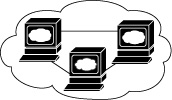
\includegraphics{Cisco_BW/web_cluster}};

\draw (LB2) -> (farm);

\node [
	start branch=1 going below right,
	diagram item,
	label=below:Http interface
] {\includegraphics{Cisco_BW/PC}};

\node [
	start branch=1 going below left,
	diagram item,
	label=below:OPC XML interface
] {\includegraphics{Cisco_BW/PC}};


\node [
	continue chain = going below,
	diagram item,
	label=below:mod Bus interface
] {\includegraphics{Cisco_BW/PC}};


\end{tikzpicture}

In this solution the load balancer needs to balance external connections to different protocols like HTTP and Modbus, however a solution witch can be extended to any restful protocol is needed. Also balancing of node roles depending on the amount incoming traffic on different interfaces will be needed.

Load balancers can also provide different features like bundling requests, security, discovering bad nodes and caching (Squid). This can offload the servers behind.

The following requirements to the system exists:
\begin{description}
	\item Robustness
	\item Protocol flexible
	\item support TCP Handoffs (for non restful applications)
	\item Must be a distributed component
\end{description}

\section{Levels of balancing}
\begin{description}
	\item[OSI 3] Network/IP %google says network layer LVS says transport layer
	\item[OSI 4] Network/IP
	\item[OSI 7] {Application level, like http balancing, allows balancing strategies based on url and user location.}
\end{description}

What we would like is a transport layer protocol.
\cite{Ludwig:SwarmIntelligenceGridLoadBalancing} Implements a particle swam based algorithm, and discuses quality parameters.

\section{Existing solutions}
\begin{description}
	\item[Linux Virtual Server: IPVS] Is implemented in the linux kernal version 2.4 and 2.6. Works at the IP level. Useed byt big sites sourceforge.net, layer 3.
	\item[Google Compute Engine: Load Balancer]: Proprietary. layer 3 and 7.
\end{description}
\chapter{Distributed computing}

As mentioned, The Wind Power Supervisor (WPS) and the Park Pilot does not scale well with the number of turbines, which forces Siemens to set the regulation cycle time after worst case scenarios (see \cref{sec:SiemensCase} for details). Today this cycle time is set to 150 ms and Siemens wants the time reduced to 10 ms. This is a major performance improvement and as such not a strict demand from the Siemens case, meaning any reduction in the 150 ms cycle time will be accepted. The goal for the decentralized solution to the Siemens case is therefore to reduce the regulation cycle time as much as possible.

Looking at the park regulation algorithm \cref{sec:SiemensCase}, the reason for it being slow is primarily the communication overhead involved, when requesting set points from every turbine and sending new set points to every turbine, and that this communication overhead increases with the number of turbines involved with the regulation. So to reduce the regulation cycle time, this communication overhead needs to be reduced, by letting each turbine perform park regulations and calculate their own set points. 

Removing the communication overhead from the regulation algorithm involves detaching sharing of data from the algorithm. In order to do this

For the Park Pilot to be able to compute a park regulation, the Park Pilot needs information about every turbine in the farm. In the same way, when decentralizing the Park Pilot, if a turbine is to compute park regulations, the turbine needs information about every other turbine. This means the windmill farm needs a global shared state, where information about every turbine in the farm is available to every turbine performing park regulations. 

%This is a major performance improvement and for that reason, performing the regulation sequence using a distributed database only is not enough, since reading/writing to the disk takes valuable milliseconds. Therefore regulation information needs to be kept in memory in order to keep regulation cycle time as low as possible. 

This chapter describes and discusses different distributed computing paradigms as a way of making a global state for the turbines to compute park regulations themselves. The goal is to find the paradigm best suited for the Siemens case. Furthermore, the chapter describes relevant technologies within the chosen paradigm and discusses which technology that is the best for the Siemens case.

The chapter uses the following definition by Andrews~\cite{andrews2000foundations} for distributed computing: \textit{In distributed computing, each node or process has its own local memory and communication happens via message passing.}



%Furthermore, when decentralizing the Wind Power Supervisor onto the turbines, the turbines obviously needs to be able to handle external data aggregation . For the heavy tasks, in terms of CPU power, distributed computing becomes relevant as a way of improving performance by combining the CPU power residing inside the turbines to compute a common task.

%
%In distributed computing, each node or process has its own local memory and communication happens via message passing~\cite{andrews2000foundations}. This means distributed computing is a way of having a global system state and keep relevant information, with regards to the global state, in memory, and thereby avoid read/write operations to the disk. 



\section{Message passing}

Message passing is a low-level communication paradigm, where processors communicate by sending messages via bidirectional channels. It is a highly used paradigm and other communication paradigms are usually implemented on top of an underlying message-passing system.  

With message passing being a low-level communication paradigm, the communication overhead is low compared to paradigms build on top of it. It is entirely up to the application developer to handle communication. This will in many cases result in better execution time, which is the most compelling argument for choosing message passing as communication paradigm. The problem with it being up to the developer, is that the developer needs to deal with configurations setup, such as sockets and marshaling, exception handling and who and when to communicate with when developing the application. This makes it hard to develop using message passing, especially when dealing with more complex applications~\cite{lu1995message}. 


\section{Distributed shared memory}

Shared memory is an attractive paradigm for designing parallel and distributed systems. Applications can use shared memory as a tool for the entire system to share a common state. However for loose coupled distributed systems, no physically shared memory is available to support such a model. Distributed shared memory (DSM) is a way of providing physically distributed memory machines a shared memory abstraction, illustrated on \cref{fig:distributedSharedMemory}.

\begin{figure}
	\centering
	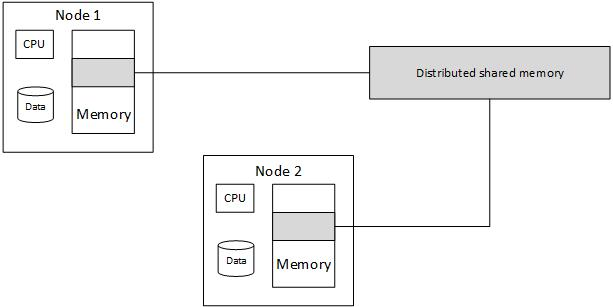
\includegraphics[width=0.8\textwidth,natwidth=610,natheight=642]{DistributedSharedMemory.jpg} 
	\captionsetup{format=plain,font=footnotesize,labelfont={bf,defaultCapFont},labelsep=quad,singlelinecheck=no}
	\caption[Distributed Computing System with 2 nodes]{
		\label{fig:distributedSharedMemory} 
		\footnotesize{%
			A distributed shared memory system with 2 nodes.
		}
	}
\end{figure}

The primary advantage of DSM is the shared memory abstraction provided. This gives the illusion of physically shared memory and allows developers to use the shared-memory paradigm, without having to think about communication mechanisms. For this reason the DSM paradigm is fully decoupled in space, since producers and consumers of data remain anonymous to each other, and in time, since the producers needs no knowledge of future use of the data. Synchronization decoupling is achieved by some implementations of DSM, where each node keeps local copies of the shared data~\cite{guedes1993distributed}.

A downside to the DSM abstraction is that it introduces overhead to the system, since the DSM abstraction has limited knowledge of the application flow, compared to communication via message passing~\cite{lu1995message}. 

 

%DSM pass by reference

%In distribted system there might be scenarios in which a task waits for a service at the queue of one resource, while at the same time another resource which is capable of serving the task is idle. The purpose of a load balancing algorithm is to prevent these scenarios as much as possible.

%three phases.
%Information collection: Gathers info of workload
%decision making: Calc optimal data dist.
%data migration: Transfer excess amount of workload from on overloaded processor to another underloaded processor

%Centralized: Size of grid increases, keppeing all the inforation about the state of all the resources is a bottlebeck. Scalability becomes an issue. Page 281. 

%The benifits of this technique stems from Load Balancing
%State Broadcast Algorithm (SBA). Page 282

%Basic assumptions Page 289.

%Scalability and makespan (Y). Page 298, conclusion.


\section{Publish/subscribe}

Publish/subscribe is a messaging pattern where communication is interest based instead of address based. Messages are characterized into classes and sent by publishers, without knowledge of how many subscribers there may be. Nodes can then subscribe to one or more classes of interest, without knowledge of how many publishers there are, providing a more decoupled, scalable and flexible interaction model.

\begin{figure}
	\centering
	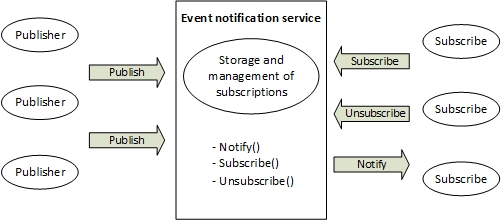
\includegraphics[width=0.9\textwidth,natwidth=610,natheight=642]{PublishSubscribe.jpg} 
	\captionsetup{format=plain,font=footnotesize,labelfont={bf,defaultCapFont},labelsep=quad,singlelinecheck=no}
	\caption[Distributed Computing System with 2 nodes]{
		\label{fig:publishSubscribe} 
		\footnotesize{%
			A simple publish/subscribe system.
		}
	}
\end{figure}

The publish/subscribe paradigm is event driven and corresponds to the observer design pattern, where subscribers are registered via keywords instead of registering their interest directly with the publishers. The paradigm relies on an event notification service providing storage and management for subscriptions and efficient delivery of events, as illustrated on \cref{fig:publishSubscribe}. The subscribers are notified subsequently of any event, generated by a publisher, matching the registered interest. The strength of this event-based communication is the full decoupling in time, space and synchronization between publishers and subscribers~\cite{eugster2003many}.

%Quality of service??

% DSM is only space and time decoupled but not sync, because consumers pull from shared space in a synchronous style


\section{Remote procedure call}

Remote procedure call (RPC) is a communications paradigm built for client/server architecture~\cite{Microsoft2003RPC}, which makes remote interactions appear the same way as local interactions. The goal is to make the process of executing code on a remote machine as simple as calling a local function~\cite{dusseau2014intro} by factoring out common tasks, such as security, synchronization, and data flow handling. This explains the paradigms popularity in distributed computing. However distribution cannot be made completely transparent to the application, because it gives rise to further types of potential failures, like communication failures, that have to be dealt with explicitly~\cite{coulouris2005distributed}. 

The idea of RPC is quite simple. When a remote procedure is invoked, the calling environment is suspended, the parameters are passed across the network to the environment where the procedure is to execute and the desired procedure is executed at that location. When execution is finished, return values are sent back to the calling environment, where execution resumes \cite{birrell1984implementing}.

A shortcoming of RPC is the strong coupling in time, space and synchronization. Although solutions have been presented to remove the synchronization coupling by future remote invocation. Remote method invocation is a paradigm where RPC as been applied to object-oriented contexts~\cite{eugster2003many}.

%Not appropriate for broadcasting

%Strong time coupled 
%sync coupled from the consumer side (waits for the return of the call, calling environment is suspended). Can be changed so sender does not expect reply (weak reliablity, no success or failure). Or return handle for sender to later request return value when needed (future remote invocation)

%Space coupling (remote reference to object)


%\section{Notification}
%
%The notification paradigm corresponds to the observer design pattern. It works by having subscribers register their interest directly with the publishers, which manages subscriptions and send events. It is usually implemented using two asynchronous invocations, in order to enforce synchronization decoupling: the first is sent by the client to the server, containing invocation arguments and a callback reference to the client, and the second is sent by the server to the client to return one or more replies. However publishers and subscribers remain coupled in time and space. Furthermore the communication management is left to the publisher. This can become a problem as the system grows in size \cite{eugster2003many}.

%Publish/Subscribe where subscribers register their interest directly with publishers, which manages subscriptions and send events.

%event driven

%\section{Message queuing}
%Message queuing is a message-centric approach that usually integrate some form of publish/subscribe transaction. It works by having producers append messages to a global FIFO or priority queue asynchronously and consumers dequeue them synchronously from that same queue, where messages can only be consumed by one consumer. At an interaction level message queues recall much of DSM, where producers feed messages to some global memory space. Similarly to DSM, producers and consumers are decoupled in both space and time, where synchronous decoupling is only present for the producers \cite{eugster2003many}.

%Global FIFO kø. Til hvis man er ligeglad med, hvem der tager opgaven??


%\begin{table}
%	\begin{tabular}{l >{\centering}m{5cm} c}
%		\hline
%		\hline
%		\textbf{Abstraction} & \textbf{Space} & \textbf{Time} & \textbf{Flow} \\
%		\hline
%		\hline
%		Message Passing & \checkmark & \checkmark \\
%		\hline
%		RPC/RMI & \checkmark & \checkmark \\
%		\hlines
%		Async. RPC/RMI & \checkmark & \checkmark \\
%		\hline
%		Future RPC/RMI & \checkmark & \checkmark \\
%		\hline
%		Notifications & \text{x}& \text{x} & \checkmark \\
%		\hline
%		DSM & \checkmark & \checkmark & P(\checkmark) \\
%		\hline
%		Message Queuing (PULL) & \checkmark & \checkmark & \text{P(} \checkmark \text{)} \\
%		\hline
%		Public/Subscribe & \checkmark & \checkmark & \checkmark \\
%		\hline
%		\hline
%	\end{tabular}
%	
%	\caption[MongoDB VoltDB]{
%		\label{tab:mongovolt}
%		\footnotesize{%
%			Comparison of MongoDB and VoltDB.
%		} 
%	}
%\end{table}

\section{Comparison with regards to the Siemens case}
Looking at the Siemens case (\cref{sec:SiemensCase}) the new distributed system must act as a single unit, be able to perform park regulations and scale easily with the number of turbines. Furthermore Siemens wish to remove single point of failures. With this in mind, the remote procedure call paradigm is not an option because it is tight coupled and build for a client/server architecture, which is exactly what Siemens is trying to avoid. One could imaging using a partial client/server architecture, with a communication hierarchy, however this would introduce some communication overhead~\cite{Yu1997JavaDSM} and single point of failures to the system.

As mentioned, to perform the park regulation sequence, the windmill farm needs a global shared state, where information about every turbine available to every turbine performing park regulations. Therefore, if the decentralized version of the Siemens case were to be implemented using raw message passing, it would result in building some kind of DSM and/or publish/subscribe abstraction, with roughly the same communication overhead. To save the trouble of developing this abstraction, we conclude that message passing is not an option as communication paradigm.

This leaves DSM and publish/subscribe as remaining paradigms, where one could imagine the Siemens case being implemented using either of the two. The abstraction of shared memory provided by DSM is attractive when looking looking at the Siemens case. As a system developer, being able to think of the global shared state as local memory is to prefer over event handling. Therefore DSM is chosen over publish/subscribe since publish/subscribe introduces event handling to the system.

% The abstraction provided by DSM is attractive when looking looking at the Siemens case. As a system developer, being able to think of the global shared state as local memory is to prefer over thinking about communication semantics. However before before choosing, it is relevant to look at the cost of the DSM abstraction.

%\subsection{Message passing or DSM?}
%
%The abstraction provided by DSM is attractive when looking looking at the Siemens case. As a system developer, being able to think of the global shared state as local memory is to prefer over thinking about communication semantics. However before before choosing, it is relevant to look at the cost of the DSM abstraction.

%Comparing DSM with message passing in terms of processing time and network communication time is not entirely fair since DSM is an abstraction built using message passing. Therefore, Honghui~\cite{lu1995message} argues that it is hard for DSM to outperform message passing, in terms of application execution time, given the larger software-overhead. Honghui has studied and compared a DSM system with message passing system, with the goal to assess the differences in application development time and program execution time between DSM and message passing, and determine the causes of the lower program execution time of DSM systems. He ported 12 different parallel program scenarios to a DSM system called TreadMarks and a message passing system called PVM. For 5 of the scenarios, TreadMarks performed within 10\% of PVM. For 6 of the programs the difference were between 10\% - 30\%. For the last scenario, PVM performed twice as well as TreadMarks. 
%
%%He ported 12 different parallel program scenarios to a DSM system called TreadMarks and a message passing system called PVM and compared the two technologies with regards to programmability and performance. He argues that given DSM is an abstraction built on top of message passing, DSM cannot achieve better performance than message passing, given the larger software-overhead. Therefore the goal is to achieve the same performance as message passing using DSM. For 5 of the scenarios, TreadMarks performed within 10\% of PVM. For 6 of the programs the difference were between 10\% - 30\%. For the last scenario, PVM performed twice as well as TreadMarks. 
%
%Honghui argues that the program execution time is dependent of the logical flow of the program scenario. More messages and more data are sent in TreadMarks, explaining the performance differences. He gives the following reasons for the extra communication in TreadMarks:
%
%\begin{itemize}
%	\item Separation of synchronization and data transfer in TreadMarks. 
%	\item Extra messages to request updates for data in the invalidate protocol used in TreadMarks.
%	\item False sharing.
%	\item Diff accumulation for migratory data in TreadMarks.
%\end{itemize} 
%
%%1) Seperation of synchronization
%% Lazy release consistency: Against data races (which may result uin wrong results). Only the next processor that acquires the lock can access x --> only that processor is informormed of the change to x --> reduce message traffic. Ex: Barriers - No processor overites values before all processors have read the value computed in the previous interation.
%
%%2) Extra messages to request updates for data in the invalidate protocol used in TreadMarks
%% Memory page change communicatin. Modified pages are inviladated after an acquire. Later access causes access miss, which in turn causes installation of an up-to-date copy of the page.
%
%%3) False sharing
%% To objects er allokerede i samme memory page og de skrives til samtidig --> force update af page --> overhead
%
%%4) diff accumulation for migratory data in TreadMarks
%% Multiple-writer protocol to allow wrinting on same page at the same time. Uses a diff algorithm to reduce false sharing effects.
%
%Honghui concludes that the performance of a well optimized DSM system is comparable to that of a message passing system. Furthermore, development of systems with complex communication patterns takes a lot less effort using the DSM paradigm.
%
%In contrast to Honghui, Stumm and Zhou~\cite{stumm1990algorithms} argues that applications using DSM can in fact outperform their message passing counterparts, in a few cases. They argue, that this is possible for the following reasons:
%
%\begin{itemize}
% 	\item DSM algorithms typically move data on demand as they are being accessed, which spreads communication load over a longer period of time, allowing for a greater degree of concurrency. If for example a node uses the shared memory more than others, the node does not need to communicate for every write operation made to the shared memory.
% 	\item For DSM algorithms that sends data in large blocks, communication overhead is reduced. 
%\end{itemize} 
%
%Looking at the Siemens case the two major factors for the communication paradigm choice are scalability and availability.
% With that in mind, BLABLA is not an option because of .. 
%
%Message queuing and RMI offers feature which  



\section{State of the art DSM}

The regulation algorithm is a recursive algorithm, which performs calculations of new turbine set points using the following parameters:

\begin{itemize}
	\item Current state of every turbine in the farm.
	\item Max capacity of each turbine.
	\item Historic data from previous calculations.
\end{itemize} 



In order to remove the communication overhead from the regulation cycle time, information sharing through the chosen paradigm, DSM, needs to to be detached from the regulation cycle. 

Looking at the global shared state 

 Removing communication overhead from the park regulation cycle involves the following

DSM is a paradigm well implemented through by many different frameworks, with their own individual and unique implementation.


Therefore, to determine which technology that is best suited for the Siemens case, the technologies will be compared on the following set of parameters: 

%standalone: Type?
%Distributed shared memory support
%Distributed shared chache support
%Distributed memeory support
%Performance
%Client/server?
%Framework architecture. distributed shared memeory, client/server or not  
%cost

With DSM chosen as the communication paradigm, this chapter describes, evaluates and discusses different DSM technologies in order to find the technology best suited for Siemens.

%Standalone, avoid overhead


\section{In memory databases}
%Client/server architecture

\section{In-memory data grids}
%Distributed memory. Only shared for replica reasons

\subsection{Oracle Coherence}
%dist. memory --> distributed chache
%java, .net, c++
%http://www.oracle.com/technetwork/middleware/coherence/distributed-caching-100021.html


\subsection{VMware Gemfire}
%Contact sales
%Not open source

\subsection{Gigaspaces XAP}
%Share nothing architecture

\subsection{ScaleOut Software}
%Java, .NET, C/C++ 
%cash
%Share nothing architecture
%http://www.scaleoutsoftware.com/downloads-resources/downloads/

\subsection{NCache}
%expensive
%http://www.alachisoft.com/ncache/index.html

\subsection{Hazelcast}
%java
%opensource
%http://hazelcast.com/products/hazelcast/

\section{Distributed shared cache}


\subsection{jBoss Cache}
%Java 5.0 and 6
%forældet


\subsection{DSM in .NET}
%IP multicast

%casusally consistent: Writes that are potentially causally related must be seen by all processes in the same order. Concurrent writes may be seen in a different order on different machines.

\subsection{AppFabric}
%Runs on IIS


\subsection{DDS}


\section{Conclusion}

%Ens
%Valg med vægt på arkitektur og development tid. 
%RMI fravalg